\chapter{WF-135 Respecting the Dojo 1000-Count Burndown}\label{record-217}

\noindent{\footnotesize\color{BookMuted}\path{docs/design/WF-135-respecting-dojo-1000.md}\par}\smallskip

\begin{RecordMeta}
title: WF-135 Respecting the Dojo 1000-Count Burndown
legend: WF
lane: bad-code
priority: high
github_issue: 374
status: complete
keywords:
  - code-dojo
  - eslint
  - standards
  - ratchet
  - respectful-repo

\end{RecordMeta}

Legend: \href{https://github.com/flyingrobots/bijou/blob/cbd70612140e7a450d764b3c7be1c6af878b99bc/docs/legends/WF-workflow-delivery.md}{WF - Workflow and Delivery}

\section{Linked Work}\label{record-217-linked-work}

\begin{itemize}
\tightlist
\item
  Issue: \href{https://github.com/flyingrobots/bijou/issues/374}{\#374}
\item
  Standards artifact: \href{https://github.com/flyingrobots/bijou/blob/cbd70612140e7a450d764b3c7be1c6af878b99bc/docs/typescript-code-standards.editors-edition.md}{TypeScript Code Standards Editor's Edition}
\item
  Exception ledger: \href{https://github.com/flyingrobots/bijou/blob/cbd70612140e7a450d764b3c7be1c6af878b99bc/docs/code-dojo-exceptions.md}{Code Dojo Exceptions}
\end{itemize}

\section{Decision Summary}\label{record-217-decision-summary}

\texttt{R\allowbreak{}e\allowbreak{}s\allowbreak{}p\allowbreak{}e\allowbreak{}c\allowbreak{}t\allowbreak{}f\allowbreak{}u\allowbreak{}l\allowbreak{} \allowbreak{}R\allowbreak{}e\allowbreak{}p\allowbreak{}o\allowbreak{}:\allowbreak{} \allowbreak{}E\allowbreak{}n\allowbreak{}t\allowbreak{}e\allowbreak{}r\allowbreak{} \allowbreak{}t\allowbreak{}h\allowbreak{}e\allowbreak{} \allowbreak{}C\allowbreak{}o\allowbreak{}d\allowbreak{}e\allowbreak{} \allowbreak{}D\allowbreak{}o\allowbreak{}j\allowbreak{}o} made the standards debt enforceable. WF-134 proved the ratchet can burn down real violations, but \texttt{m\allowbreak{}a\allowbreak{}i\allowbreak{}n} still has thousands of counted exceptions. This cycle raises the bar from minimum 50-count goalpost reductions to a 1000-count burndown pass.

The long-term goal is uncompromising:

\begin{itemize}
\tightlist
\item
  zero ESLint errors
\item
  zero Code Dojo warnings, errors, or issues
\item
  zero files violating length restrictions
\end{itemize}

This cycle is not allowed to move that goalpost by weakening rules, excluding files, or raising baselines.

\section{Sponsored Human}\label{record-217-sponsored-human}

A maintainer wants the repository to stop treating the standards as symbolic and make a visible move toward real compliance.

\section{Sponsored Agent}\label{record-217-sponsored-agent}

An agent needs a concrete large burndown target, live count evidence, and clear guardrails so cleanup work stays reviewable instead of becoming a broad semantic rewrite.

\section{Hill}\label{record-217-hill}

Reduce aggregate Code Dojo debt from \texttt{4\allowbreak{},\allowbreak{}9\allowbreak{}4\allowbreak{}0} to \texttt{3\allowbreak{},\allowbreak{}9\allowbreak{}4\allowbreak{}0} or lower with real cleanup. Lower the official ratchet ceilings to the new live counts so future work cannot regain the violations.

\section{Scope}\label{record-217-scope}

\begin{itemize}
\tightlist
\item
  Target high-yield, mechanically reviewable ESLint clusters first:

  \begin{itemize}
  \tightlist
  \item
    non-null assertions that can become local guards or reusable helpers
  \item
    unsafe \texttt{a\allowbreak{}n\allowbreak{}y} and unsafe assertion clusters in tests and scripts
  \item
    template-expression findings with explicit string formatting
  \item
    stale async wrappers and unused values where the fix is local
  \end{itemize}
\item
  Reduce file/context debt when touched files exceed the current threshold.
\item
  Keep changes clustered by surface so validation can be focused.
\item
  Update \texttt{s\allowbreak{}c\allowbreak{}r\allowbreak{}i\allowbreak{}p\allowbreak{}t\allowbreak{}s\allowbreak{}/\allowbreak{}c\allowbreak{}o\allowbreak{}d\allowbreak{}e\allowbreak{}-\allowbreak{}d\allowbreak{}o\allowbreak{}j\allowbreak{}o\allowbreak{}/\allowbreak{}b\allowbreak{}a\allowbreak{}s\allowbreak{}e\allowbreak{}l\allowbreak{}i\allowbreak{}n\allowbreak{}e\allowbreak{}s\allowbreak{}/\allowbreak{}e\allowbreak{}s\allowbreak{}l\allowbreak{}i\allowbreak{}n\allowbreak{}t\allowbreak{}.\allowbreak{}j\allowbreak{}s\allowbreak{}o\allowbreak{}n}, \texttt{d\allowbreak{}o\allowbreak{}c\allowbreak{}s\allowbreak{}/\allowbreak{}c\allowbreak{}o\allowbreak{}d\allowbreak{}e\allowbreak{}-\allowbreak{}d\allowbreak{}o\allowbreak{}j\allowbreak{}o\allowbreak{}-\allowbreak{}e\allowbreak{}x\allowbreak{}c\allowbreak{}e\allowbreak{}p\allowbreak{}t\allowbreak{}i\allowbreak{}o\allowbreak{}n\allowbreak{}s\allowbreak{}.\allowbreak{}m\allowbreak{}d}, and \texttt{p\allowbreak{}a\allowbreak{}c\allowbreak{}k\allowbreak{}a\allowbreak{}g\allowbreak{}e\allowbreak{}.\allowbreak{}j\allowbreak{}s\allowbreak{}o\allowbreak{}n} only after live counts prove the reduction.
\end{itemize}

\section{Non-Goals}\label{record-217-non-goals}

\begin{itemize}
\tightlist
\item
  Do not disable, soften, or narrow ESLint rules.
\item
  Do not raise any Code Dojo ceiling.
\item
  Do not exclude files from Code Dojo or ESLint.
\item
  Do not make risky product behavior changes for static-analysis convenience.
\item
  Do not split mega-files purely by line count unless the ownership boundary is obvious and tests can cover the move.
\end{itemize}

\section{Current Evidence}\label{record-217-current-evidence}

Live counts on \texttt{m\allowbreak{}a\allowbreak{}i\allowbreak{}n} at \texttt{e\allowbreak{}d\allowbreak{}4\allowbreak{}3\allowbreak{}8\allowbreak{}e\allowbreak{}b\allowbreak{}e}:

\begin{itemize}
\tightlist
\item
  aggregate Code Dojo debt: \texttt{4\allowbreak{},\allowbreak{}9\allowbreak{}4\allowbreak{}0}
\item
  ESLint findings: \texttt{4\allowbreak{},\allowbreak{}5\allowbreak{}1\allowbreak{}7}
\item
  ESLint errors: \texttt{4\allowbreak{},\allowbreak{}5\allowbreak{}1\allowbreak{}3}
\item
  ESLint warnings: \texttt{4}
\item
  file/context baseline: \texttt{3\allowbreak{}4\allowbreak{}2}
\item
  mock-ban baseline: \texttt{2\allowbreak{}3}
\item
  code-size baseline: \texttt{5\allowbreak{}8}, including \texttt{4} legacy hard-limit files
\end{itemize}

Top ESLint rules:

\begin{center}
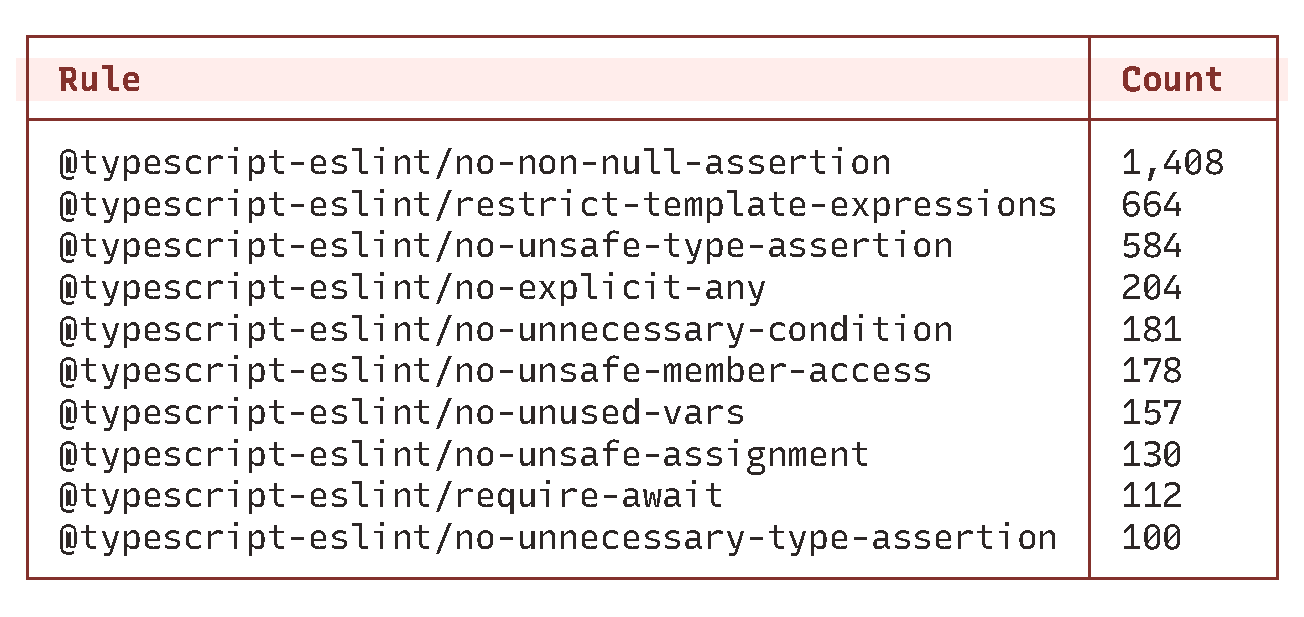
\includegraphics[width=\linewidth]{figures/tables/table-045-g1-1.pdf}
\par\smallskip{\scriptsize\color{BookMuted}Rows 1–10. Actual Bijou table component.}
\end{center}


\section{Playback Questions}\label{record-217-playback-questions}

\begin{enumerate}
\def\labelenumi{\arabic{enumi}.}
\tightlist
\item
  Did aggregate Code Dojo debt fall to \texttt{3\allowbreak{},\allowbreak{}9\allowbreak{}4\allowbreak{}0} or lower?
\item
  Did the stored ESLint baseline match the new live count?
\item
  Did file/context and code-size debt hold or shrink?
\item
  Did touched behavioral surfaces get focused validation?
\item
  Does \texttt{n\allowbreak{}p\allowbreak{}m\allowbreak{} \allowbreak{}r\allowbreak{}u\allowbreak{}n\allowbreak{} \allowbreak{}c\allowbreak{}o\allowbreak{}d\allowbreak{}e\allowbreak{}-\allowbreak{}d\allowbreak{}o\allowbreak{}j\allowbreak{}o\allowbreak{}:\allowbreak{}c\allowbreak{}i} pass after the lower ceiling is installed?
\end{enumerate}

\section{Tests To Write First}\label{record-217-tests-to-write-first}

Pure static-analysis rewrites use the existing lint finding as RED and the lower live count as GREEN. Add focused regression tests before changing runtime behavior, helper contracts, parsing, scheduling, schema normalization, or user visible rendering.

\section{Acceptance Criteria}\label{record-217-acceptance-criteria}

\begin{itemize}
\tightlist
\item
  Aggregate Code Dojo debt is \texttt{3\allowbreak{},\allowbreak{}9\allowbreak{}4\allowbreak{}0} or lower.
\item
  \texttt{s\allowbreak{}c\allowbreak{}r\allowbreak{}i\allowbreak{}p\allowbreak{}t\allowbreak{}s\allowbreak{}/\allowbreak{}c\allowbreak{}o\allowbreak{}d\allowbreak{}e\allowbreak{}-\allowbreak{}d\allowbreak{}o\allowbreak{}j\allowbreak{}o\allowbreak{}/\allowbreak{}b\allowbreak{}a\allowbreak{}s\allowbreak{}e\allowbreak{}l\allowbreak{}i\allowbreak{}n\allowbreak{}e\allowbreak{}s\allowbreak{}/\allowbreak{}e\allowbreak{}s\allowbreak{}l\allowbreak{}i\allowbreak{}n\allowbreak{}t\allowbreak{}.\allowbreak{}j\allowbreak{}s\allowbreak{}o\allowbreak{}n} records the lower live ESLint count and per-rule counts.
\item
  \texttt{d\allowbreak{}o\allowbreak{}c\allowbreak{}s\allowbreak{}/\allowbreak{}c\allowbreak{}o\allowbreak{}d\allowbreak{}e\allowbreak{}-\allowbreak{}d\allowbreak{}o\allowbreak{}j\allowbreak{}o\allowbreak{}-\allowbreak{}e\allowbreak{}x\allowbreak{}c\allowbreak{}e\allowbreak{}p\allowbreak{}t\allowbreak{}i\allowbreak{}o\allowbreak{}n\allowbreak{}s\allowbreak{}.\allowbreak{}m\allowbreak{}d} reports the lower aggregate debt count and next target.
\item
  \texttt{p\allowbreak{}a\allowbreak{}c\allowbreak{}k\allowbreak{}a\allowbreak{}g\allowbreak{}e\allowbreak{}.\allowbreak{}j\allowbreak{}s\allowbreak{}o\allowbreak{}n} lowers \texttt{c\allowbreak{}o\allowbreak{}d\allowbreak{}e\allowbreak{}-\allowbreak{}d\allowbreak{}o\allowbreak{}j\allowbreak{}o\allowbreak{}:\allowbreak{}d\allowbreak{}e\allowbreak{}b\allowbreak{}t\allowbreak{} \allowbreak{}-\allowbreak{}-\allowbreak{}m\allowbreak{}a\allowbreak{}x} to the new live aggregate count.
\item
  Focused tests for touched clusters pass.
\item
  \texttt{n\allowbreak{}p\allowbreak{}m\allowbreak{} \allowbreak{}r\allowbreak{}u\allowbreak{}n\allowbreak{} \allowbreak{}c\allowbreak{}o\allowbreak{}d\allowbreak{}e\allowbreak{}-\allowbreak{}d\allowbreak{}o\allowbreak{}j\allowbreak{}o\allowbreak{}:\allowbreak{}c\allowbreak{}i}, \texttt{n\allowbreak{}p\allowbreak{}m\allowbreak{} \allowbreak{}r\allowbreak{}u\allowbreak{}n\allowbreak{} \allowbreak{}d\allowbreak{}o\allowbreak{}c\allowbreak{}s\allowbreak{}:\allowbreak{}i\allowbreak{}n\allowbreak{}v\allowbreak{}e\allowbreak{}n\allowbreak{}t\allowbreak{}o\allowbreak{}r\allowbreak{}y}, and \texttt{g\allowbreak{}i\allowbreak{}t\allowbreak{} \allowbreak{}d\allowbreak{}i\allowbreak{}f\allowbreak{}f\allowbreak{} \allowbreak{}-\allowbreak{}-\allowbreak{}c\allowbreak{}h\allowbreak{}e\allowbreak{}c\allowbreak{}k} pass before final review.
\end{itemize}

\section{Retrospective}\label{record-217-retrospective}

Completed with a measured aggregate Code Dojo debt reduction from \texttt{4\allowbreak{},\allowbreak{}9\allowbreak{}4\allowbreak{}0} to \texttt{2\allowbreak{},\allowbreak{}0\allowbreak{}6\allowbreak{}8} (\texttt{-\allowbreak{}2\allowbreak{},\allowbreak{}8\allowbreak{}7\allowbreak{}2}). The stored ESLint baseline now records \texttt{1\allowbreak{},\allowbreak{}6\allowbreak{}5\allowbreak{}6} live findings, down from \texttt{4\allowbreak{},\allowbreak{}5\allowbreak{}1\allowbreak{}7} (\texttt{-\allowbreak{}2\allowbreak{},\allowbreak{}8\allowbreak{}6\allowbreak{}1}), and the next aggregate target is \texttt{2\allowbreak{},\allowbreak{}0\allowbreak{}1\allowbreak{}8} or lower. Follow-on passes covered mechanically reviewable clusters across tests, scripts, examples, MCP docs, DOGFOOD, app-frame surfaces, render/surface helpers, table/markdown parsing, geometry, benchmarks, runtime helpers, i18n helpers, and TUI input/action surfaces.

The latest pass removed app-frame action/input-shell assertion debt, bench CLI formatting debt, focus-map text formatting debt, key parser regex/assertion debt, and node style test regex debt. Touched file/context budgets stayed below their stored ceilings, two file/context exceptions have been removed, and the latest app-frame core/overlay pass removed retained-layout non-null assertions, shell-command handler narrowing casts, combo-key formatting debt, and framed-app runtime bridge assertions. The binding cluster then removed runtime brand casts, unchecked generic snapshot casts, descriptor clone assertions, and unchecked fixture casts from the core binding contract and tests. The runtime/schema cluster removed TUI runtime binding brand casts, command dispatch narrowing debt, schema-block brand casts, schema bind-output assertions, and extracted inert schema data cloning into a focused helper.

